\documentclass[border=10pt]{standalone}

\usepackage{tikz}
\usepackage{tikzsymbols}
\usetikzlibrary{calc,patterns,shapes.geometric}

\def\centerarc[#1](#2)(#3:#4:#5){\draw[#1] ($(#2)+({#5*cos(#3)},{#5*sin(#3)})$) arc (#3:#4:#5);}

\begin{document}
	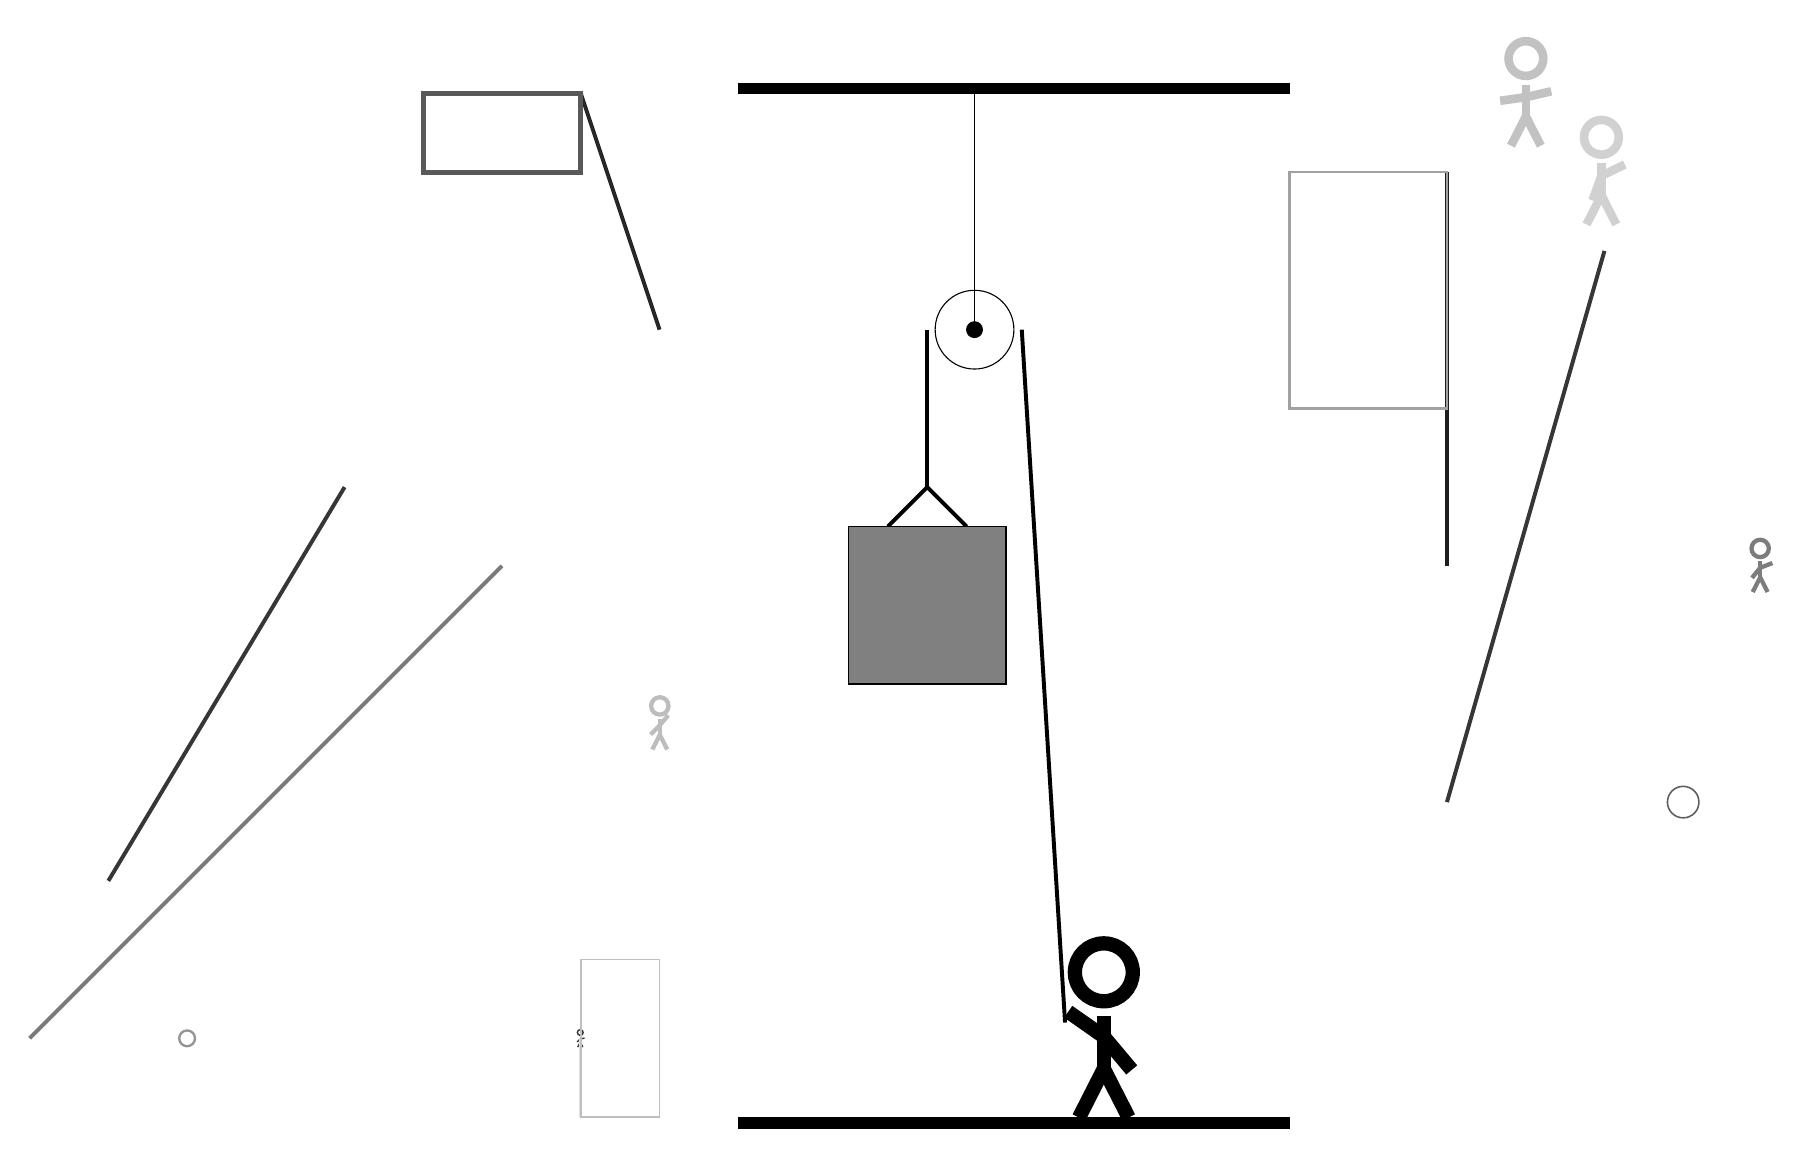
\begin{tikzpicture}
		%%%%% START %%%%%
		
		\draw[fill=black] (-2, 10) rectangle (5, 10.125);
		
		\draw (1, 7) circle (0.5);
		\draw[fill=black] (1, 7) circle (0.1);
		\draw (1, 10) -- (1, 7);
		
		\draw[line width=0.5mm] (-0.1, 4.5) -- (0.4, 5.0) -- (0.9, 4.5);
		\draw[fill=black!50] (-0.6, 4.5) rectangle (1.4, 2.5);
		
		\draw[line width=0.5mm] (0.4, 7) -- (0.4, 5.0);
		\centerarc[line width=0.5mm](1, 7)(0:180:0.6);
		\draw[line width=0.5mm](1.6, 7) -- (2.15, -1.8);
		
		\node at (2.6, -1.9) {\Strichmaxerl[10][-35][-50]};
		
		\draw [line width=0.2mm, color=black!63](10, 1) circle (0.2);
		
		\draw[line width=0.4mm, color=black!88] (7, 4) rectangle (7, 9);
		\draw[line width=0.3mm, color=black!37] (7, 6) rectangle (5, 9);
		\node[line width=0.7mm, color=black!79] at (-4, -2) {\Strichmaxerl[1][43][11]};
		
		\node[line width=0.6mm, color=black!26] at (-3, 2) {\Strichmaxerl[3][45][50]};
		\node[line width=0.6mm, color=black!51] at (11, 4) {\Strichmaxerl[3][51][21]};
		\draw[line width=0.4mm, color=black!13] (-4, -3) rectangle (-4, -2);
		\draw [line width=0.3mm, color=black!42](-9, -2) circle (0.1);
		\draw[line width=0.5mm, color=black!79](9, 8) -- (7, 1);
		\node[line width=0.2mm, color=black!24] at (8, 10) {\Strichmaxerl[6][8][13]};
		\draw[line width=0.2mm, color=black!25] (-3, -3) rectangle (-4, -1);
		\node[line width=0.4mm, color=black!18] at (9, 9) {\Strichmaxerl[6][70][26]};
		\draw[line width=0.5mm, color=black!79](-7, 5) -- (-10, 0);
		
		\draw[line width=0.5mm, color=black!85](-3, 7) -- (-4, 10);
		\draw[line width=0.5mm, color=black!52](-5, 4) -- (-11, -2);
		\draw[line width=0.6mm, color=black!65] (-4, 9) rectangle (-6, 10);
		
		\draw[fill=black] (-2, -3) rectangle (5, -3.15);
		
		%%%%% END %%%%%
	\end{tikzpicture}
\end{document}